%%%%%%%%%%%%%%%%%%%%%%%%%%%%%%%%%%%%%%%%%
% University/School Laboratory Report
% LaTeX Template
% Version 3.0 (4/2/13)
%
% This template has been downloaded from:
% http://www.LaTeXTemplates.com
%
% Original author:
% Linux and Unix Users Group at Virginia Tech Wiki 
% (https://vtluug.org/wiki/Example_LaTeX_chem_lab_report)
%
% License:
% CC BY-NC-SA 3.0 (http://creativecommons.org/licenses/by-nc-sa/3.0/)
%
%%%%%%%%%%%%%%%%%%%%%%%%%%%%%%%%%%%%%%%%%

%----------------------------------------------------------------------------------------
%	PACKAGES AND DOCUMENT CONFIGURATIONS
%----------------------------------------------------------------------------------------

\documentclass{article}

\usepackage{mhchem} % Package for chemical equation typesetting
\usepackage{siunitx} % Provides the \SI{}{} command for typesetting SI units

\usepackage{graphicx} % Required for the inclusion of images
\usepackage[utf8]{inputenc}
\usepackage{CJK}

\setlength\parindent{0pt} % Removes all indentation from paragraphs

\renewcommand{\labelenumi}{\alph{enumi}.} % Make numbering in the enumerate environment by letter rather than number (e.g. section 6)
\newcommand{\tabincell}[2]
{
	\begin{tabular}
	{@{}#1@{}}#2
	\end{tabular}
}

%\usepackage{times} % Uncomment to use the Times New Roman font

%----------------------------------------------------------------------------------------
%	DOCUMENT INFORMATION
%----------------------------------------------------------------------------------------

\title{Determination of the Atomic \\ Weight of Magnesium \\ CHEM 101} % Title

\author{John \textsc{Smith}} % Author name

\date{\today} % Date for the report

\begin{document}
\begin{CJK*}{UTF8}{gkai}

\maketitle % Insert the title, author and date

\begin{center}
\begin{tabular}{l r}
Date Performed: & January 1, 2012 \\ % Date the experiment was performed
Partners: & James Smith \\ % Partner names
& Mary Smith \\
Instructor: & Professor Smith % Instructor/supervisor
\end{tabular}
\end{center}

% If you wish to include an abstract, uncomment the lines below
% \begin{abstract}
% Abstract text
% \end{abstract}

%----------------------------------------------------------------------------------------
%	SECTION 1
%----------------------------------------------------------------------------------------

\section{Objective}

To determine the atomic weight of magnesium via its reaction with oxygen and to study the stoichiometry of the reaction (as defined in \ref{definitions}):\\

\begin{center}\ce{2 Mg + O2 -> 2 MgO}\end{center}

% If you have more than one objective, uncomment the below:
%\begin{description}
%\item[First Objective] \hfill \\
%Objective 1 text
%\item[Second Objective] \hfill \\
%Objective 2 text
%\end{description}

\subsection{Definitions}
\label{definitions}
\begin{description}
\item[Stoichiometry]
The relationship between the relative quantities of substances taking part in a reaction or forming a compound, typically a ratio of whole integers.
\item[Atomic mass]
The mass of an atom of a chemical element expressed in atomic mass units. It is approximately equivalent to the number of protons and neutrons in the atom (the mass number) or to the average number allowing for the relative abundances of different isotopes. 
\end{description} 
 
%----------------------------------------------------------------------------------------
%	SECTION 2
%----------------------------------------------------------------------------------------

\section{Experimental Data}

\begin{tabular}{ll}
Mass of empty crucible & \SI{7.28}{g}\\
Mass of crucible and magnesium before heating & \SI{8.59}{g}\\
Mass of crucible and magnesium oxide after heating & \SI{9.46}{g}\\
Balance used & \#4\\
Magnesium from sample bottle & \#1
\end{tabular}

%----------------------------------------------------------------------------------------
%	SECTION 3
%----------------------------------------------------------------------------------------

\section{Sample Calculation}

\begin{tabular}{ll}
Mass of magnesium metal & = \SI{8.59}{g} - \SI{7.28}{g}\\
& = \SI{1.31}{g}\\
Mass of magnesium oxide & = \SI{9.46}{g} - \SI{7.28}{g}\\
& = \SI{2.18}{g}\\
Mass of oxygen & = \SI{2.18}{g} - \SI{1.31}{}\\
& = \SI{0.87}{g}
\end{tabular}\\
Because of this reaction, the required ratio is the atomic weight of magnesium: \SI{16.00}{g} of oxygen as experimental mass of Mg: experimental mass of oxygen or $\frac{x}{1.31}=\frac{16}{0.87}$ from which, $M_{\ce{Mg}} = 16.00 \times \frac{1.31}{0.87} = 24.1 = \SI{24}{g/mol}$ (to two significant figures).

%----------------------------------------------------------------------------------------
%	SECTION 4
%----------------------------------------------------------------------------------------

\section{Results and Conclusions}

The atomic weight of magnesium is concluded to be \SI{24}{g/mol}, as determined by the stoichiometry of its chemical combination with oxygen. This result is in agreement with the accepted value.

\begin{figure}[h]
\begin{center}
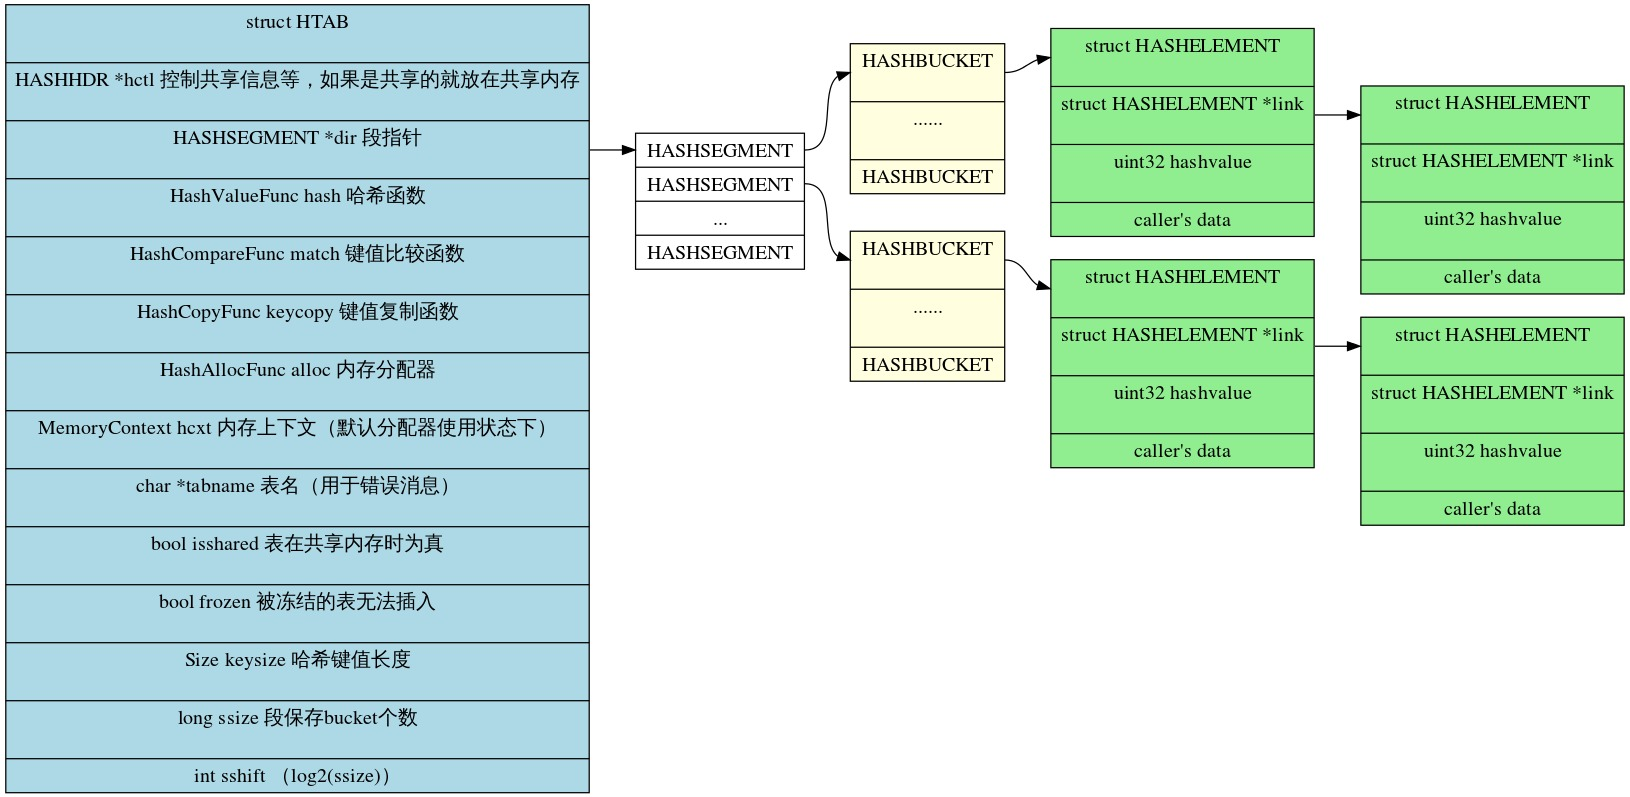
\includegraphics[width=0.65\textwidth]{hash.jpg} % Include the image placeholder.png
\caption{Figure caption.}
\end{center}
\end{figure}

%----------------------------------------------------------------------------------------
%	SECTION 5
%----------------------------------------------------------------------------------------

\section{Discussion of Experimental Uncertainty}

The accepted value (periodic table) is \SI{24.3}{g/mol} \cite{Smith:2012qr}. The percentage discrepancy between the accepted value and the result obtained here is 1.3\%. Because only a single measurement was made, it is not possible to calculate an estimated standard deviation. \\

The most obvious source of experimental uncertainty is the limited precision of the balance. Other potential sources of experimental uncertainty are: the reaction might not be complete; if not enough time was allowed for total oxidation, less than complete oxidation of the magnesium might have, in part, reacted with nitrogen in the air (incorrect reaction); the magnesium oxide might have absorbed water from the air, and thus weigh ``too much." Because the result obtained is close to the accepted value it is possible that some of these experimental uncertainties have fortuitously cancelled one another.

%----------------------------------------------------------------------------------------
%	SECTION 6
%----------------------------------------------------------------------------------------

\section{Answers to Definitions}

\begin{enumerate}
\begin{item}
The \emph{atomic weight of an element} is the relative weight of one of its atoms compared to C-12 with a weight of 12.0000000$\ldots$, hydrogen with a weight of 1.008, to oxygen with a weight of 16.00. Atomic weight is also the average weight of all the atoms of that element as they occur in nature.
\end{item}
\begin{item}
The \emph{units of atomic weight} are two-fold, with an identical numerical value. They are g/mole of atoms (or just g/mol) or amu/atom.
\end{item}
\begin{item}
\emph{Percentage discrepancy} between an accepted (literature) value and an experimental value is $\frac{|\mathrm{experimental result} - \mathrm{accepted result}|}{\mathrm{accepted result}}$.
\end{item}
\end{enumerate}

%----------------------------------------------------------------------------------------
%	BIBLIOGRAPHY
%----------------------------------------------------------------------------------------

\bibliographystyle{unsrt}

\bibliography{sample}

%----------------------------------------------------------------------------------------



%\documentclass{article}
%
%\usepackage{mhchem}
%\usepackage{siunitx}
%\setlength\parindent{1pt}
%\renewcommand{\labelenumi}{\alph{enumi}.}
%%\setbeamerfont{block title}{size={}}
%%\setbeamercolor{titlelike}{parent=structure,bg=white}
%%\setbeamertemplate{navigation symbols}{}
%\usepackage[utf8]{inputenc}
%\usepackage{CJK}
%\usepackage{verbatim}
%\usepackage{graphicx}
%\usepackage{multirow}
%%\hypersetup{CJKbookmarks=true}
%\usepackage[T1]{fontenc}
%\newcommand{\tabincell}[2]
%{
%	\begin{tabular}
%	{@{}#1@{}}#2
%	\end{tabular}
%}
%
%\title{Postgresql 存储管理中的HASH}
%\author{马文韬}
%\date{\today}
%%\institute{WHU}
%
%
%
%\begin{document}
%\begin{CJK*}{UTF8}{gkai}
%\maketitle
%



\section{概述}
\begin{figure}[!ht]
\centering
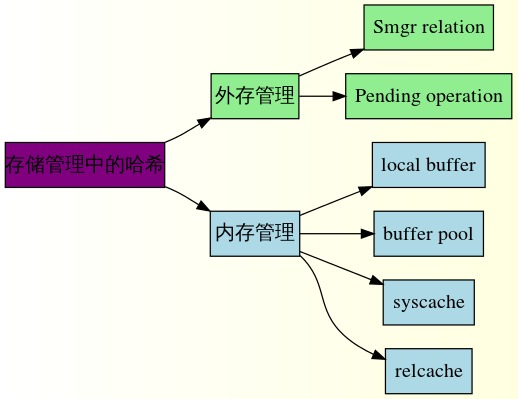
\includegraphics[width = 100mm]{index.jpg}
\caption{存储管理中的哈希图}
\label{overflow}
\end{figure}

\section{Hash table基本结构及其操作} 
asdfadsgsagasdg

\begin{figure}[!ht]
\begin{center}
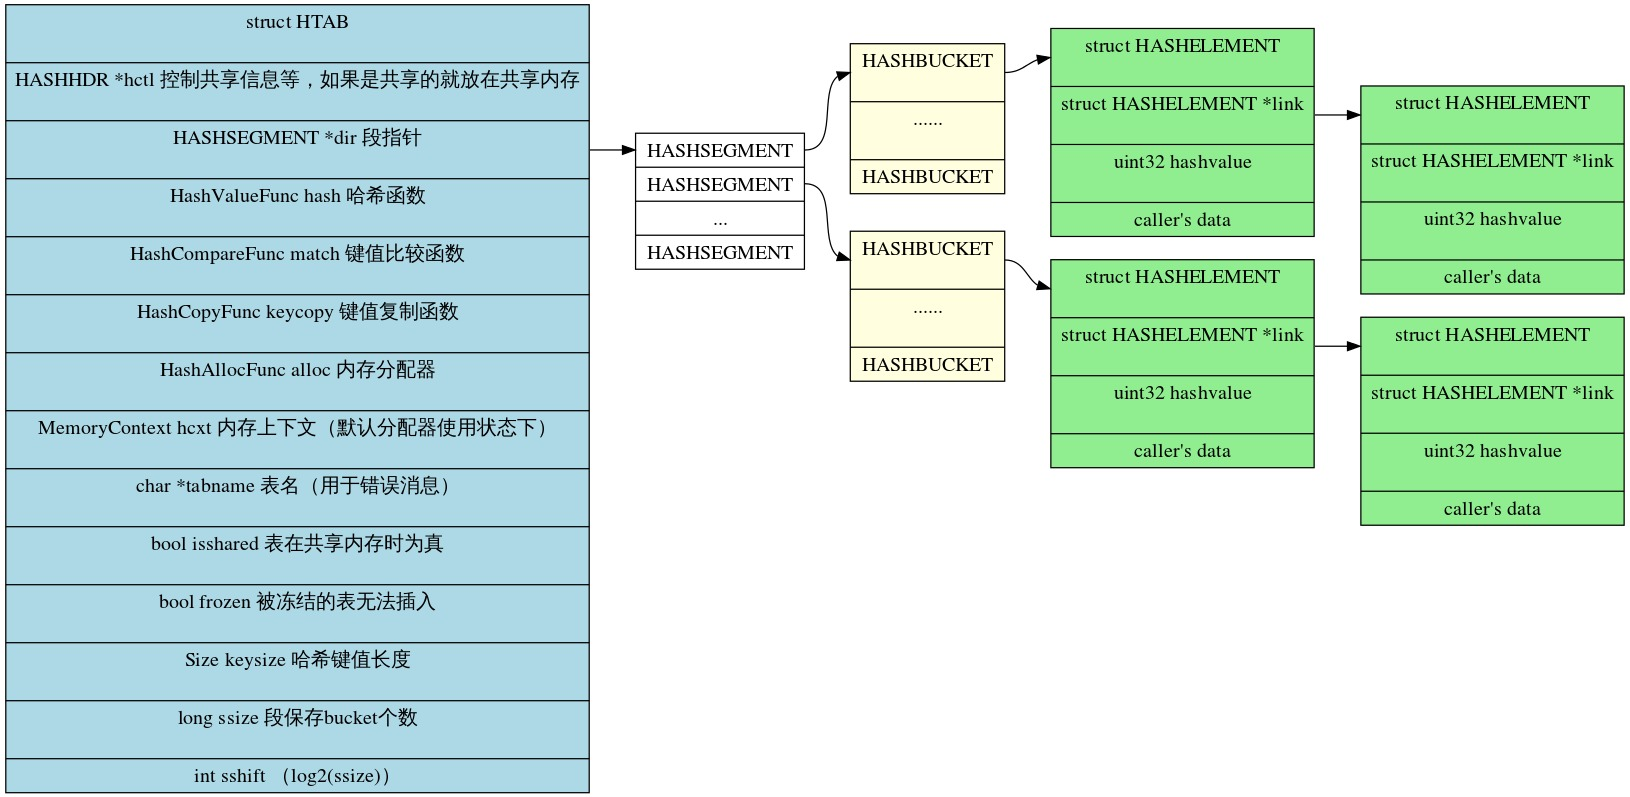
\includegraphics[width=0.7\textwidth]{hash.jpg}
\caption{hash table 结构图}
\end{center}
\end{figure}

asdfasd
%\begin{figure}[ht!]
%\begin{tabular}{cc}
%\begin{minipage}[t]{2in}
%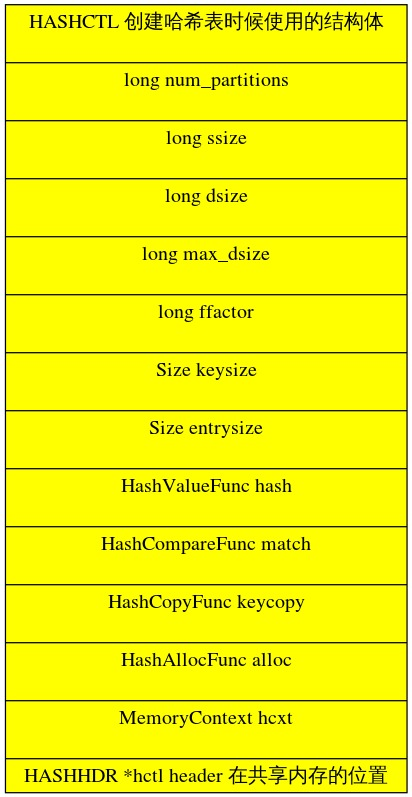
\includegraphics[height = 60mm]{hashctl.jpg}
%\caption{HASHCTL结构图}
%\end{minipage}
%%
%\begin{minipage}[t]{2in}
%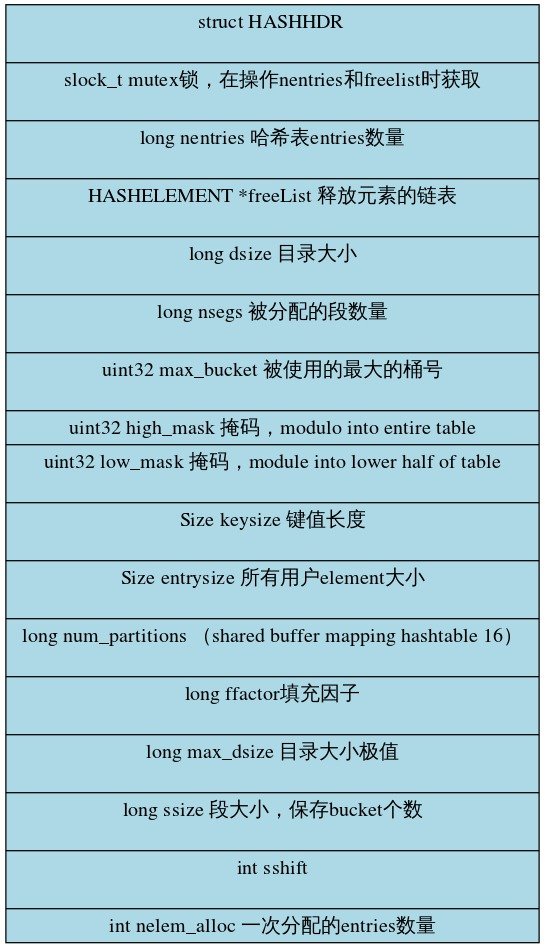
\includegraphics[height = 60mm]{hashhdr.jpg}
%\caption{HASHHDR结构图}
%\end{minipage}
%\end{tabular}
%\end{figure}

%HASHHDR 存在于共享内存中,每个后端还有一个对应的本地HTAB结构,对应非共享哈希表,HASHHDR和HTAB功能上没有区别。\\
\begin{table}
\scriptsize
\centering
\caption{哈希结构体中函数指针的默认函数及其功能}
\label{address}
\begin{tabular}{|c|c|}
\hline
函数指针  &  相关函数 \\
\hline
HashValueFunc hash & 
\tabincell{c}{ string\_hash 计算string哈希值\\tag\_hash 计算tag哈希值\\oid\_hash 计算oid的哈希值\\bitmap\_hash计算bitmap哈希}\\
\hline
HashCompareFunc match & \tabincell{c}{ string\_compare,如果不自定义,默认\\bitmap\_match 和bitmap\_hash一起用}\\
\hline
HashCopyFunc keycopy & \tabincell {c}{strlcpy 可以自定义,默认}\\
\hline
HashAllocFunc alloc  & \tabincell{c}{DynaHashAlloc  调用上下文\\中定义的内存分配方法}\\
\hline
\end{tabular}
\end{table}


%\begin{table}
%\centering
%\caption{HashValueFucn类型}
%\begin{tabular}{|c|c|}
%\hline
%函数名称  &  函数用途 \\
%\hline
%string\_hash & \tabincell{c}{计算strings的哈希值 }\\
%\hline
%tag\_hash  & \tabincell{c}{计算固定大小\\tag的哈希值}\\
%\hline
%oid\_hash & \tabincell {c}{key是OID,计算哈希}\\
%\hline
%bitmap\_hash & \tabincell{c}{key是bitmap集}\\
%\hline
%bitmap\_match  & \tabincell{c}{和bitmap\_hash一起用,\\用作match函数}\\
%\hline
%\end{tabular}
%\end{table}


%\begin{table}
%\caption{哈希函数表}
%\begin{tabular}{|c|c|c|}
%\hline 
%函数名 &  主要参数  &  功能 \\
%\hline
%hash\_create & \tabincell{c}{表名,大小,\\HASHCTL结构\\第三个参数标记位} &\tabincell{c}{创建一个动\\态哈希表}\\
%\hline
%hash\_search & \tabincell{c}{哈希表指针,键指针,\\ action标记,\\指向查询结果指针} & \tabincell{c}{对哈希表进行查找,\\插入,删除等操作}\\
%\hline
%\end{tabular}
%\end{table}
%

%\tiny void *hash\_search(HTAB *hashp,   void *keyPtr,   HASHACTION action,   bool *foundPtr);
\begin{table}
\caption{hash\_search相关操作action标记}
\begin{tabular}{|c|c|c|}
\hline
 HASH\_FIND & \tabincell{c}{ 根据key\\查找哈希表} \\
\hline
 HASH\_ENTER & \tabincell{c}{ 查找哈希表,\\如果entry没出现,\\那么创建一个 }\\
\hline
 HASH\_ENTER\_NULL & \tabincell{c}{查找哈希表,\\如果超出内存,\\返回NULL}  \\
\hline
 HASH\_REMOVE &\tabincell{c} {移除有特定key的entry} \\
\hline
\end{tabular}
\end{table}


\section{Smgr relation中的Hash} 
\tiny
\begin{itemize}
\item \quad Oid spcNode; 表空间
\item \quad Oid dbNode ; 数据库
\item \quad Oid relNode; 关系
\end{itemize}


\begin{figure}[!ht]
\centering
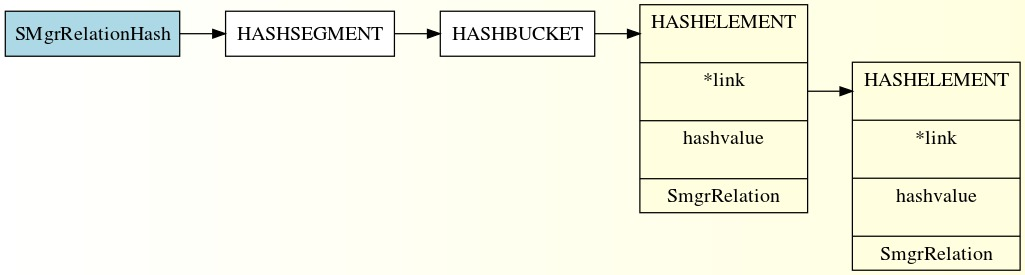
\includegraphics[width = 100mm]{smgr.jpg}
\caption{smgr中的哈希}
\label{overflow}
\end{figure}


\begin{table}
\tiny
\caption{smgr relation中的哈希函数}
\begin{tabular}{|c|c|c|c|}
\hline
\tabincell{c}{函数名}  &
\tabincell{c}{参数}  &
\tabincell{c}{调用函数} &
\tabincell{c}{使用场景}\\
\hline
\tabincell{c}{hash\_search}&
\tabincell{c}{SMgrRelationHash,\\(void *)\&rnode,\\HASH\_ENTER,\&found}&
\tabincell{c}{SMgrRelation  \\smgropen(RelFileNode rnode)}&
\tabincell{c}{RelFileNode作为主键\\查找并返回SMgrRelation对象,\\找不到就创建一个}\\
\hline
\tabincell{c}{hash\_search}&
\tabincell{c}{SMgrRelationHash,\\\&(reln->smgr\_rnode),\\HASH\_REMOVE,NULL}&
\tabincell{c}{void \\smgrclose(SMgrRelation reln)}&
\tabincell{c}{smgr关系的RelFileNode\\作为主键查找并删除\\SMgrRelation对象}\\
\hline
\tabincell{c}{hash\_search}&
\tabincell{c}{SMgrRelationHash,\\(void *)\&rnode\\HASH\_FIND,NULL}&
\tabincell{c}{ void \\smgrclosenode(RelFileNode rnode)}&
\tabincell{c}{RelFileNode作为主键查找返回\\相应SMgrRelation对象,\\由smgrclose完成删除\\避免创建无用关系}\\
\hline
\end{tabular}
\end{table}


\section{Pending operation中的Hash} 

\tiny
\begin{itemize}
\item \quad PendingOperationTag;
\item \quad bool canceled;
\item \quad CycleCtr cycle\_ctr;
\end{itemize}

\tiny
\begin{itemize}
\item \quad RelFileNode rnode;
\item \quad ForkNumber forkNum;
\item \quad BlockNumber  segno;
\end{itemize}



\begin{figure}[!ht]
\centering
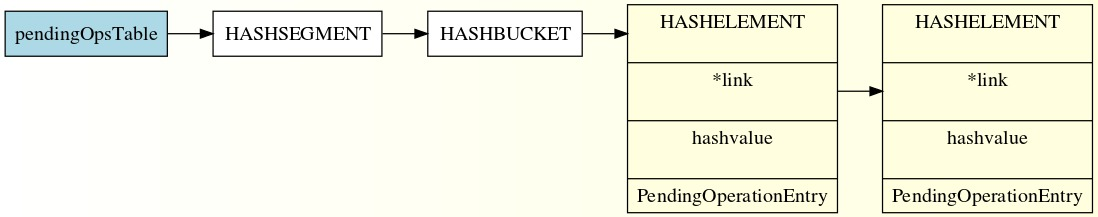
\includegraphics[width = 100mm]{pending.jpg}
\caption{pending operation中的哈希}
\label{overflow}
\end{figure}


\begin{table}
\tiny
\caption{pending operation中的哈希函数}
\begin{tabular}{|c|c|c|c|}
\hline
\tabincell{c}{函数名}  &
\tabincell{c}{参数}  &
\tabincell{c}{调用函数} &
\tabincell{c}{使用场景}\\
\hline
\tabincell{c}{hash\_search}&
\tabincell{c}{pendingOpsTable,\\\&entry->tag,\\HASH\_REMOVE,\\NULL}&
\tabincell{c}{void mdsync(void)}&
\tabincell{c}{写操作同步到磁盘时\\删除已经无效的操作\\,PendingOperationTag\\作为键查找相应操作并移除}\\
\hline
\tabincell{c}{hash\_search}&
\tabincell{c}{pendingOpsTable,\\\&key,HASH\_ENTER,\\\&found}&
\tabincell{c}{void RememberFsyncRequest\\(RelFileNode rnode,\\ForkNumber forknum,\\BlockNumber segno)}&
\tabincell{c}{PendingOperationTag作为\\主键将fsync的请求\\添加到哈希表中}\\
\hline
\end{tabular}
\end{table}



\section{SysCache中的Hash} 
\begin{figure}[ht!]
\centering
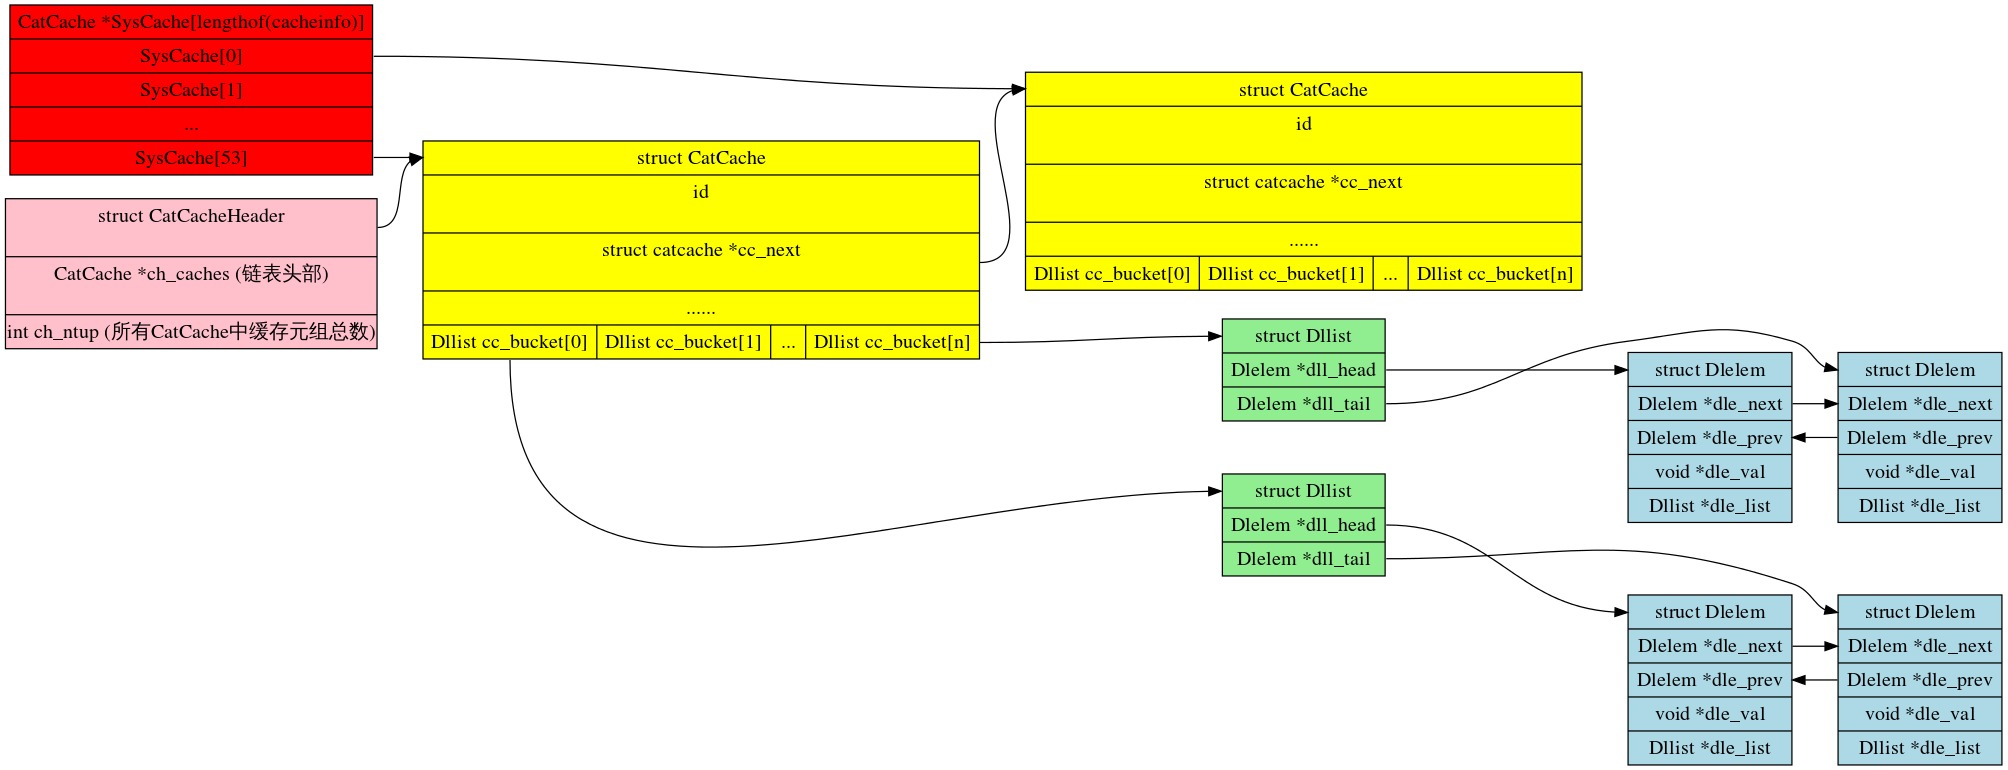
\includegraphics[width = 110mm]{syscache.jpg}
\caption{hash桶结构图}
\label{overflow}
\end{figure}



\begin{table}
\scriptsize
\caption{精确匹配基本流程及相关函数}
\begin{tabular}{|c|c|}
\hline
初始化关键字信息 & \tabincell{c}{根据四个关键字初始化cur\_skey}\\
\hline
计算哈希值和索引 & \tabincell{c} {CatalogCacheComputeHashValue\\
				由关键字计算hashValue\\
				HASH\_INDEX宏利用hashValue\\
				和cc\_buckets计算索引}\\
\hline
在索引对应的桶中查找 & \tabincell{c}{HeapKeyTest检查key是否匹配\\
				    将匹配的元组移动到链表头}\\
\hline

\end{tabular}
\end{table}


\begin{table}
\scriptsize
\centering
\caption{部分匹配基本流程及相关函数}
\begin{tabular}{|c|c|}
\hline
初始化关键字信息 & \tabincell{c}{根据部分关键字初始化cur\_skey}\\
\hline
计算哈希值和索引 & \tabincell{c} {CatalogCacheComputeHashValue\\
				根据关键字个数计算lhashValue}\\
\hline
\tabincell{c}{在CatCache的cc\_lists\\指向的CatCList链表中查找}         & \tabincell{c}{HeapKey					Test检查key是否匹配\\
		         	将匹配的CatClist放到cc\_lists\\
			 	链表的头部\\
			 	不存在CatCList,扫描物理表并构建}\\
\hline
\end{tabular}
\end{table}




\section{RelCache中的Hash} 

\tiny
Relation 的Oid作为key进行查询。

\begin{figure}[!ht]
\centering
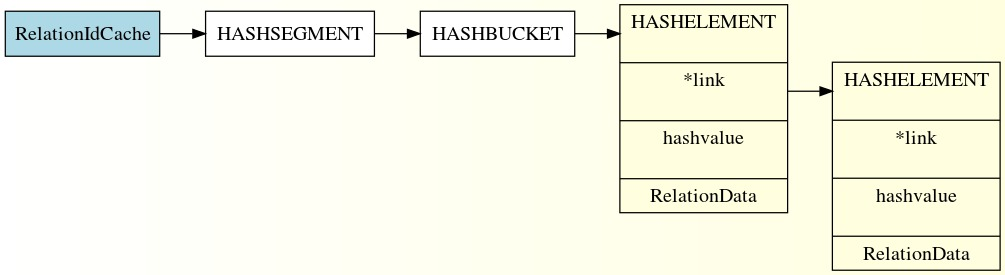
\includegraphics[width = 100mm]{rel.jpg}
\caption{relcache中的哈希}
\label{overflow}
\end{figure}

\begin{table}
\tiny
\caption{RelCache中的hash}
\begin{tabular}{|c|c|c|c|}
\hline
\tabincell{c}{函数名}  &
\tabincell{c}{参数}  &
\tabincell{c}{调用宏} &
\tabincell{c}{使用场景}\\
\hline
\tabincell{c}{hash\_search}&
\tabincell{c}{RelationIdCache,\\\&(RELATION->rd\_id),\\HASH\_ENTER\\,\&found}  &
\tabincell{c}{RelationCacheInsert\\(RELATION)} &
\tabincell{c}{以关系的Oid作为\\主键将新的关系\\插入到relcache\\哈希表中}\\
\hline
\tabincell{c}{hash\_search}&
\tabincell{c}{RelationIdCache,\\\&(ID),HASH\_FIND,\\NULL}  &
\tabincell{c}{RelationIdCacheLookup\\(ID,RELATION)}&
\tabincell{c}{用关系Oid作为主键\\在relcache中查找相应对象}\\
\hline
\tabincell{c}{hash\_search}&
\tabincell{c}{RelationIdCache,\\\&(RELATION->rd\_id),\\HASH\_REMOVE,\\NULL}&
\tabincell{c}{RelationCacheDelete\\(RELATION)}&
\tabincell{c}{用关系Oid作为\\主键查找并删除\\relcache相应对象}\\
\hline
\end{tabular}
\end{table}


%\begin{table}
%\caption{共享缓冲区内存分配部分}
%\begin{tabular}{|c|c|c|}
%\hline
%\tabincell{c}{函数名}  &
%\tabincell{c}{调用函数} &
%\tabincell{c}{使用场景}\\
%\hline
%\tabincell{c}{hash\_create\\(ENTER)}&
%\tabincell{c}{ShemeInitHash} &
%\tabincell{c}{在共享内存(ShemeIndex)\\中创建并且\\初始化或者追加\\一个哈希表。}\\
%\hline
%\tabincell{c}{hash\_search \\(ENTER\_NULL)}&
%\tabincell{c}{ShmemInitStruct}&
%\tabincell{c}{在共享内存哈希表中初始化\\或者查找一个数据结构}\\
%\hline
%\tabincell{c}{hash\_search \\(REMOVE)}&
%\tabincell{c}{ShmemInitStruct}&
%\tabincell{c}{添加结构时内存溢出,\\移除相应结构}\\
%\hline
%\end{tabular}
%\end{table}
%
%



\section{Buffer pool中的Hash} 

\begin{itemize}
\item \quad rnode(表空间OID,数据库OID和表OID组成);\\
\item \quad forkNum 枚举类型,标记缓冲区中文件块类型;\\
\item \quad blockNum  块号;
\end{itemize}

\begin{figure}[!ht]
\centering
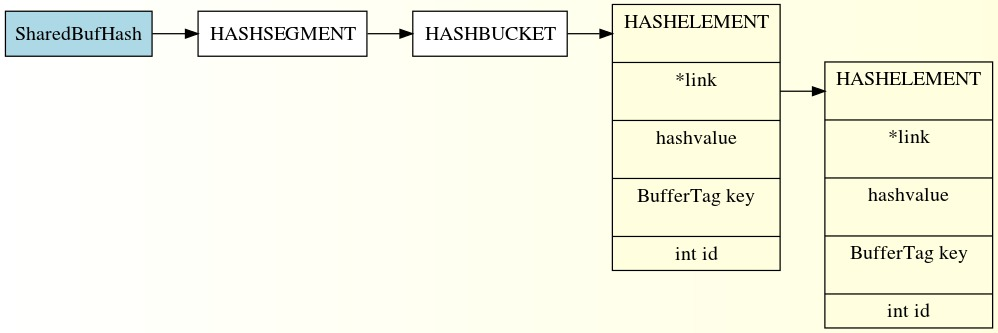
\includegraphics[width = 100mm]{buf.jpg}
\caption{}
\label{overflow}
\end{figure}


\begin{table}
\tiny
\caption{buffer pool中的hash}
\begin{tabular}{|c|c|c|c|}
\hline
\tabincell{c}{函数名}  &
\tabincell{c}{参数}  &
\tabincell{c}{调用函数} &
\tabincell{c}{使用场景}\\
\hline
\tabincell{c}{hash\_search\_with\\\_hash\_value}&
\tabincell{c}{SharedBufHash,\\tagPtr,\\hashcode,\\HASH\_FIND,\\NULL}&
\tabincell{c}{int BufTableLookup\\(BufferTag *tagPtr,\\uint32 hashcode)} &
\tabincell{c}{根据BufferTag\\在ShareBufHash中查询,\\返回buffer ID}\\
\hline
\tabincell{c}{hash\_search\_with\\\_hash\_value}&
\tabincell{c}{SharedBufHash,\\tagPtr,\\hashcode,\\HASH\_REMOVE,\\NULL}&
\tabincell{c}{void BufTableDelete\\(BufferTag *tagPtr,uint32 hashcode)}&
\tabincell{c}{根据BufferTag删除\\ShareBufHash中的entry}\\
\hline
\tabincell{c}{hash\_search\_with\\\_hash\_value}&
\tabincell{c}{SharedBufHash,\\tagPtr,\\hashcode,\\HASH\_ENTER,\\\&found}&
\tabincell{c}{int BufTableInsert(BufferTag *tagPtr,\\uint32 hashcode,\\int buf\_id}&
\tabincell{c}{根据BufferTag和\\buffer ID插入entry,\\如果有冲突entry,\\返回冲突entry的buffer ID}\\
\hline
\end{tabular}
\end{table}




\section{Local buffer中的Hash} 

和buffer pool一样,使用BufferTag作为键进行查找。
\begin{figure}[!ht]
\centering
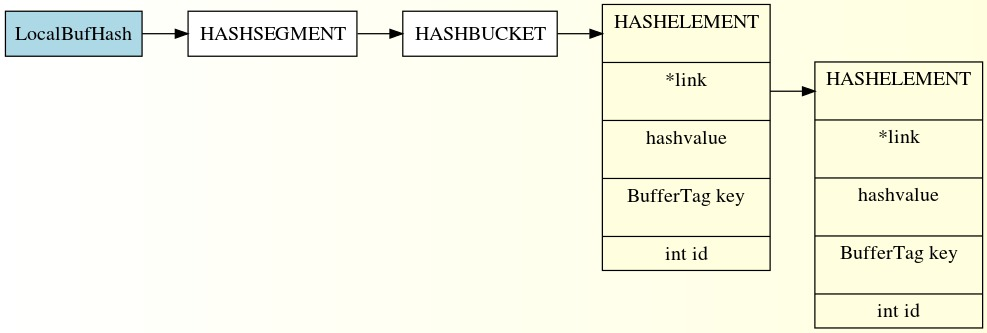
\includegraphics[width = 100mm]{local.jpg}
\caption{local buffer中的哈希}
\label{overflow}
\end{figure}

\begin{table}
\tiny
\caption{local buffer中的哈希函数}
\begin{tabular}{|c|c|c|c|}
\hline
\tabincell{c}{函数名}  &
\tabincell{c}{参数}  &
\tabincell{c}{调用函数} &
\tabincell{c}{使用场景}\\
\hline
\tabincell{c}{hash\_search}&
\tabincell{c}{LocalBufHash,\&newTag,\\HASH\_FIND,NULL}  &
\tabincell{c}{void LocalPrefetchBuffer\\(SMgrRelation smgr,\\ForkNumber forkNum,\\BlockNumber blockNum)} &
\tabincell{c}{异步读取一个关系块\\用smgr等参数创建一个tag,\\查找LocalBufHash中相应块}\\
\hline
\tabincell{c}{hash\_search}&
\tabincell{c}{LocalBufHash,\&newTag,\\HASH\_FIND,NULL}  &
\tabincell{c}{void LocalBufferAlloc\\(SMgrRelation smgr,\\ForkNumber forkNum,\\BlockNumber blockNum,\\bool *foundPtr)} &
\tabincell{c}{用smgr等参数创建一个tag,\\为给定关系的给定页面创建\\local buffer}\\
\hline
\tabincell{c}{hash\_search}&
\tabincell{c}{LocalBufHash,\\\&bufHdr->tag,\\HASH\_REMOVE,NULL}  &
\tabincell{c}{void LocalBufferAlloc\\(SMgrRelation smgr,\\ForkNumber forkNum,\\BlockNumber blockNum,\\bool *foundPtr)} &
\tabincell{c}{更新LocalBufHash,\\移除旧的entry}\\
\hline
\tabincell{c}{hash\_search}&
\tabincell{c}{LocalBufHash,\\\&bufHdr->tag,\\HASH\_ENTER,NULL}  &
\tabincell{c}{void LocalBufferAlloc\\(SMgrRelation smgr,\\ForkNumber forkNum,\\BlockNumber blockNum,\\bool *foundPtr)} &
\tabincell{c}{更新LocalBufHash,\\创建新的entry}\\
\hline
\end{tabular}
\end{table}






\end{CJK*}
\end{document}





